\section{Filtering}

The number of points delivered to the modelling component in the raw point clouds is huge. Therefore filtering out non-interesting points is required such that the workload can be kept within an acceptable range. A cut-off filter can be used to create a region of interest (ROI) and a voxel-grid filter can be used for down-sampling and to obtain equal sampling density, however the disadvantage is that the down-sampling means loss of information, and therefore there is a trade off between speed and level of detail in the reconstruction process.  

\begin{figure}[htb]
	\begin{center}
		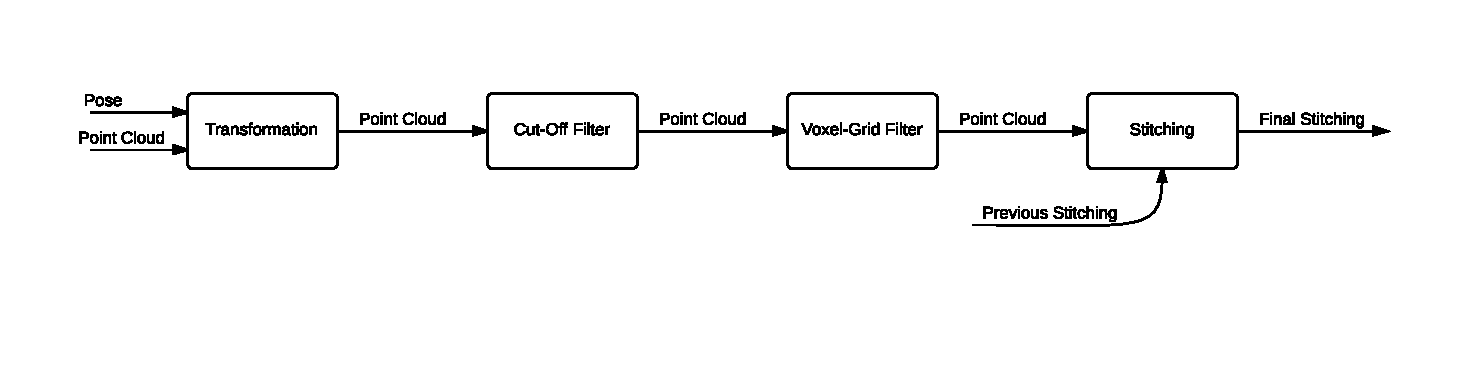
\includegraphics[scale=0.6,trim=20 70 0 20]{graphics/07_modelling/FilterFlow.pdf}%trim=l b r t
		\caption{Illustrates the flow through the filter.}
		\label{fig:filter_flow}
	\end{center}
\end{figure}

In figure \ref{fig:filter_flow} an illustration of the flow through the filter can be seen. The vision layer is delivering one point cloud for each viewpoint and along with it a pose of the camera frame at that viewpoint. The point clouds are transformed to a common frame based on the camera pose in a ROS node also handling the cut-off and voxel filtering and finally stitching them together in a combined cloud. This combined cloud, when finished, is sent to the reconstruction layer. In the sections below a brief description of the components shown in figure \ref{fig:filter_flow} is given. 

\subsection{Point cloud library}
The Point Cloud Library (PCL) utilised in this project is a library providing functionality for working with 3D point clouds. PCL delivers a variety of functionality such as filters, segmentation, surface reconstruction, kd-trees, octrees, visualisation, etc. PCL can be found at http://www.pointclouds.org/, along with documentation and tutorials.

\subsection{Point cloud transformation}
Messages received from the vision layer needs to be processed before filtering. This is because the messages delivered to the modelling component contain a point cloud and a pose of the current camera view. The coordinates of the individual points in the cloud are related to the camera frame, but this frame is moving around the object so a transformation of points is needed such they can be related a common static frame.

\begin{figure}[htb]
	\begin{center}
		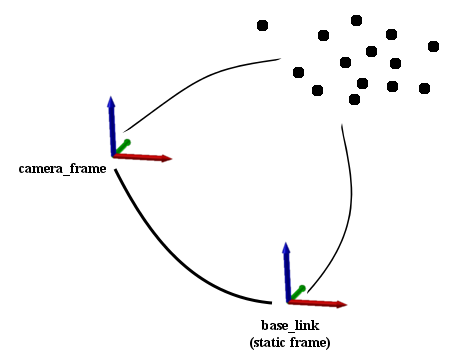
\includegraphics[scale=0.7,trim=0 0 0 0]{graphics/07_modelling/pctransform.png}%trim=l b r t
		\caption{Illustrates points in different frames.}
		\label{fig:filtering_transform}
	\end{center}
\end{figure}

\subsection{Cut-off filter}
The cut-off filter utilised is the implementation from PCL, \texttt{pcl::PassThrough< \ldots >}. A cut-off filter is utilised to create a ROI in the transformed point cloud, partly because the number of points needs to be reduced with respect to processing time and then because the region in which the object resides is fairly small compared to the region recorded by the camera.

\subsection{Voxel-grid filter}
The voxel-grid down-samples the output from cut-off filtering. The down-sampling causes loss of information which mean that surface details are lost in the process, so the amount of down-sampling must be chosen with respect to processing time versus level of detail to be reconstructed. The PCL library holds an implementation of a voxel-filter (\texttt{pcl::VoxelGrid< \ldots >}) that is utilised in the filtering node.\\

The voxel-grid filter works by splitting down the ROI into smaller regions (voxels) of a certain resolution and each point in the cloud is assigned to a voxel. Figure \ref{fig:filtering_voxel_grid} show the principle of the voxel-grid. A new point is approximated based on each voxel based on the centroid of the points contained in the voxel. This method is a little slower compared to just placing the new point in the center of the voxel, but it helps save some more detailed information about the surface curvature.
\begin{figure}[htb]
	\begin{center}
		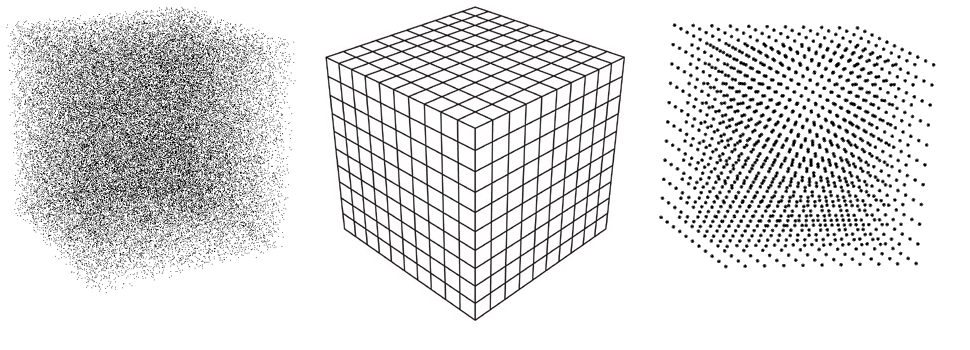
\includegraphics[scale=0.4,trim=0 0 0 0]{graphics/07_modelling/voxelgrid.png}%trim=l b r t
		\caption{Illustrates the down sampling principle of the voxel-grid filter. The left point cloud is down sampled through a set of virtual cubes, which leaves the right cloud after processing the input. A uniform distribution of points is obtained this way for instance.}
		\label{fig:filtering_voxel_grid}
	\end{center}
\end{figure}

\subsection{Point cloud stitching}
%Leon replaced: The individual point clouds from the individual views of the object are passed through the filter, the individual cloud is then stitched into another common cloud which is assembled from a number of individual clouds, predetermined by the decision making layer. The stitching of each cloud happens in the static frame, due to the transformation of the input to the filter node. The point clouds are stitched in the order at which they are received, thus the first frame becomes a sort of reference frame for the following frames. This is because the algorithm used for stitching the clouds together actually calculates a transform at which new incoming point clouds are transformed. The algorithm utilised for stitching is Iterative Closest Point (ICP). This is also implemented in in PCL and therefore this implementation (\texttt{pcl::IterativeClosestPointNonLinear< \ldots , \ldots >}) of the algorithm utilised.

The point clouds are transformed to the base frame and the first point cloud to arrive is used as reference. The following clouds are aligned to the reference using Iterative Closest Point(ICP), combined with the reference and finally the reference is down-sampled in a voxel-filter.\\ 

A version of the ICP algorithm using Levenberg-Marquardt and quaternion optimisation\cite{Rusinkiewicz} is implemented in PCL (\texttt{pcl::IterativeClosestPointNonLinear< \ldots , \ldots >}). The ICP algorithm is only guaranteed to find local maxima and as such depends on the previous alignment being relatively good, which is fulfilled by the transformation to base frame. Furthermore if a cloud is not aligned correctly, this will cause an error to propagate through to the following clouds leading to a rather distorted model of the object of interest\cite{choe2007registration}. The ICP algorithm implicitly makes the assumption of correspondence between neighbouring points and furthermore assumes that the following error is normally distributed with zero mean.

\subsection{Results}
Preliminary results of the point cloud stitching is shortly presented and discussed here. 

\begin{figure}[htb]
	\centering
        \begin{subfigure}[b]{0.4\textwidth}
        \begin{center}
			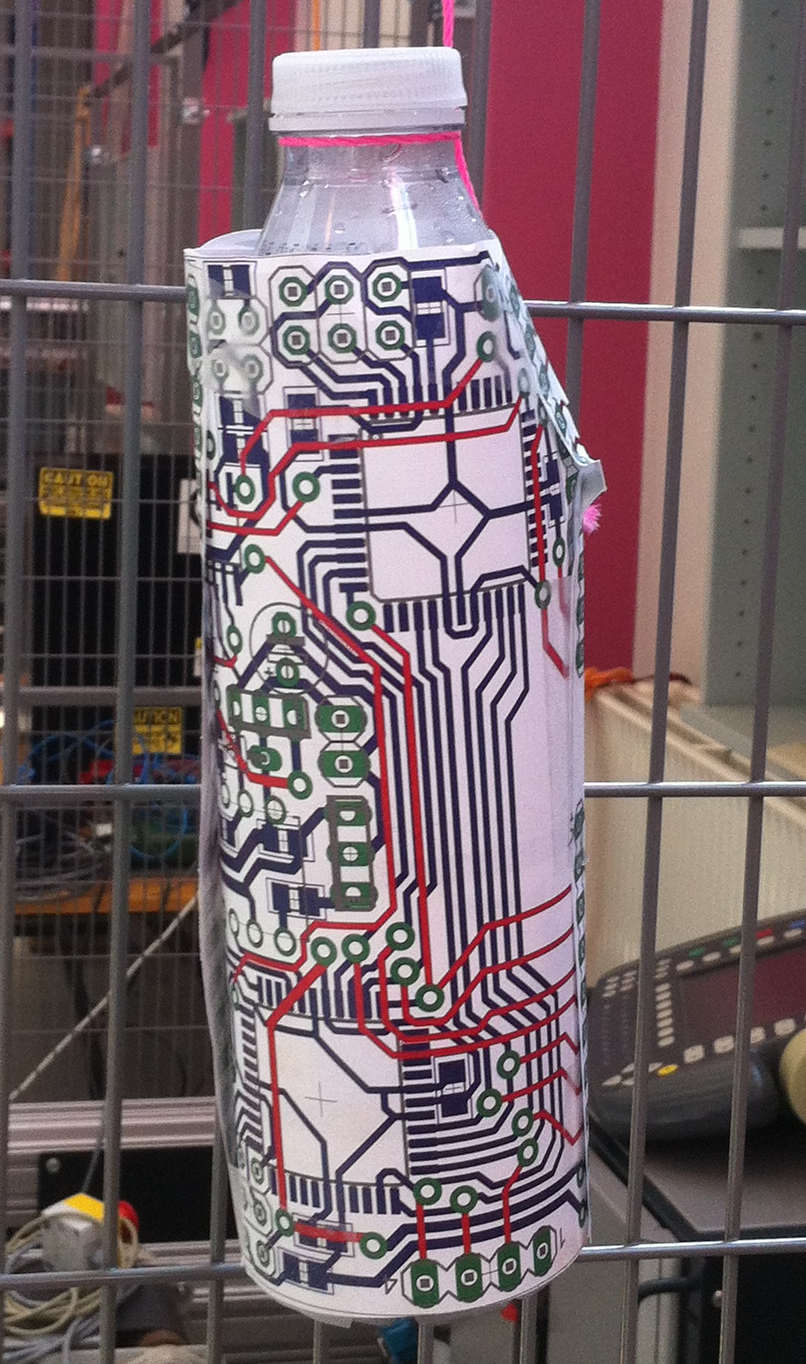
\includegraphics[width=0.6\textwidth]{graphics/07_modelling/bottle_image.png}
			\end{center}
        \end{subfigure}
        \begin{subfigure}[b]{0.4\textwidth}
        \begin{center}
			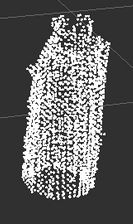
\includegraphics[width=0.6\textwidth]{graphics/07_modelling/bottle.png}
			\end{center}
        \end{subfigure}  
		\caption{Image and stitched point cloud of the bottle. (Carmine data).}\label{fig:bottle}
\end{figure}

\noindent As seen in figure \ref{fig:bottle} the stitching seems reasonable compared to the image. Inspecting the stitching further reveals a layered structure due to bad alignment as seen in figure \ref{fig:bottle_slice}.

\begin{figure}[htb]
	\begin{center}
		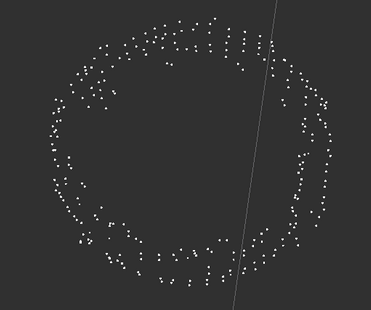
\includegraphics[scale=0.7,trim=0 0 0 0]{graphics/07_modelling/slice.png}%trim=l b r t
		\caption{Illustrates a slice of the stitching seen in figure \ref{fig:bottle}. (Carmine data).}
		\label{fig:bottle_slice}
	\end{center}
\end{figure}

\noindent The slice of the stitching seen in figure \ref{fig:bottle_slice} indicates that the alignment of the individual point clouds is not perfect. This can be due to uncertainties in the sensing or unfulfilled assumptions. It is suggested that measuring uncertainties and non-calibrated frames are creating the effect seen in slice of the bottle.\\